\documentclass[
	classe=$1^{ere}STI2D$,gray
]{exercice}

\usepackage{diagbox}
\usetikzlibrary{calc}

\renewcommand{\arraystretch}{1.4}

\title{Exercice : sondage}
\author{}
\date{}

% #1 = position
% #2 = list
% #3 = size
\newcounter{piegraphpercentcount}
\newcommand{\piegraph}[3]{%
	\draw #1 circle (#3); 
	\setcounter{piegraphpercentcount}{0}
	\coordinate (Coord2) at ($#1 + (0,#3)$);

	\foreach \data/\percent/\color in #2 {
		\pgfmathsetmacro\piegraphpercentcountbis{\thepiegraphpercentcount + \percent / 2}
		\pgfmathsetmacro\startangle{\thepiegraphpercentcount/100*360 + 90}
		\addtocounter{piegraphpercentcount}{\percent}
		\pgfmathsetmacro\endangle{\thepiegraphpercentcount/100*360 + 90}
		
		\pgfmathsetmacro\tx{cos(\endangle)*#3}
		\pgfmathsetmacro\ty{sin(\endangle)*#3}
		\coordinate (Coord1) at (Coord2);
		\coordinate (Coord2) at ($#1 + (\tx,\ty)$);

		\draw[fill=\color] #1 -- (Coord1) arc (\startangle:\endangle:#3) -- #1;

		\pgfmathsetmacro\tx{cos(\piegraphpercentcountbis/100*360 + 90)*#3/2}
		\pgfmathsetmacro\ty{sin(\piegraphpercentcountbis/100*360 + 90)*#3/2}
		\node at ($#1 + (\tx,\ty)$) {\data \\ $\percent$ \%};
	}
}

\begin{document}

\maketitle

Pour réaliser un exposé, des élèves de première cherchent des informations sur Internet. Pour trouver leur informations, ils utilisent soit une tablette, soit un téléphone, soit un ordinateur portable. Voici les résultats d'un sondage réalisé simultanément en France (500 personnes) et au Danemark (150 personnes) sur l'appareil utilisé.

\begin{center}
	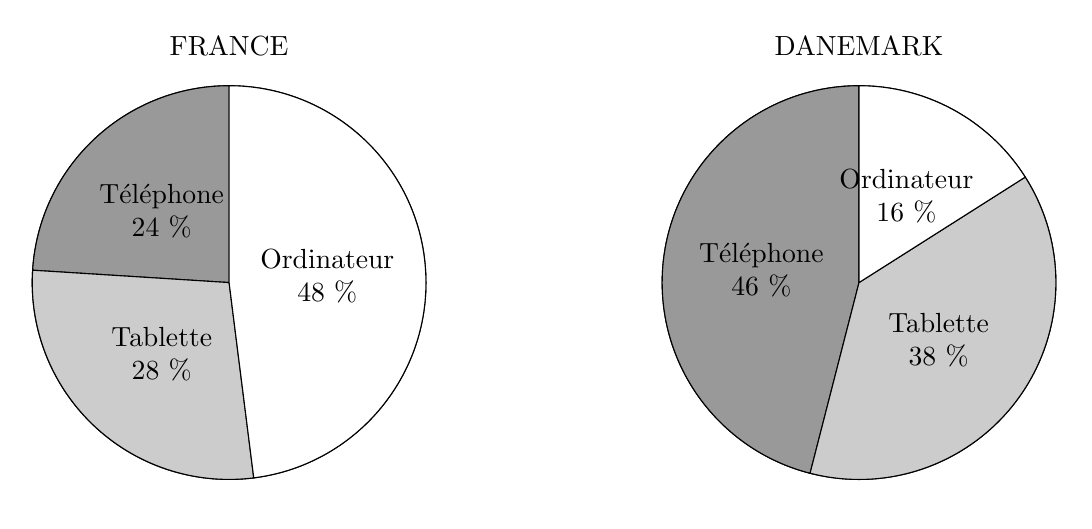
\begin{tikzpicture}[every text node part/.style={align=center}]
		\node at (0,3) {FRANCE};
		\piegraph{(0,0)}{{Téléphone/24/black!40,Tablette/28/black!20,Ordinateur/48/white}}{2.5}
		\node at (8,3) {DANEMARK};
		\piegraph{(8,0)}{{Téléphone/46/black!40,Tablette/38/black!20,Ordinateur/16/white}}{2.5}
	\end{tikzpicture}
\end{center}

\begin{enumerate}
	\item Compléter le tableau d'\textbf{effectifs} suivant :
	      \begin{center}
		      \begin{tabular}{|l|*{3}{>{\centering}p{2cm}|}}
			      \hline
			      \diagbox{$X =$ appareil}{$Y =$ pays} & France           & Danemark         & TOTAL \tabularnewline \hline
			      Téléphone                            & \correction{120} & \correction{69}  & \correction{189}\tabularnewline \hline
			      Tablette                             & \correction{140} & \correction{57}  & \correction{197}\tabularnewline \hline
			      Ordinateur                           & \correction{240} & \correction{24}  & \correction{264} \tabularnewline \hline
			      TOTAL                                & \correction{500} & \correction{150} & \correction{650}\tabularnewline \hline
		      \end{tabular}
	      \end{center}
	\item Peut-on dire que l'effectif des élèves utilisant leur téléphone est plus important au Danemark qu'en France ?

	      \correctionDots{Oui : 120 élèves utilisent leur téléphone en France, contre 69 au Danemark}
	\item On choisit au hasard un élève en France ou au Danemark. Sachant que cet élève utilise son téléphone, calculer la probabilité qu'il soit français.

	      \correctionDots{189 élèves au total utilisent leur téléphone. On doit donc calculer $\frac{120}{189} = 63,5\%$}
	\item Établir le tableau des fréquences par rapport à l'effectif global :

	      \ifdefined\makeCorrection
		      {\color{red}}
		      \begin{center}
			      \begin{tabular}{|l|*{3}{>{\centering}p{2cm}|}}
				      \hline
				      \diagbox{$X =$ appareil}{$Y =$ pays} & France  & Danemark & TOTAL \tabularnewline \hline
				      Téléphone                            & 18,5 \% & 10,6 \%  & 29,1 \% \tabularnewline \hline
				      Tablette                             & 21,5 \% & 8,8 \%   & 30,3 \% \tabularnewline \hline
				      Ordinateur                           & 36,9 \% & 3,7 \%   & 40,6 \% \tabularnewline \hline
				      TOTAL                                & 76,9 \% & 23,1 \%  & 100 \% \tabularnewline \hline
			      \end{tabular}
		      \end{center}
	      \fi
\end{enumerate}

\end{document}